\subsection{Математична модель}

Під час проєктування та аналізу систем обробки зображень виникає фундаментальна необхідність у їх строгому математичному описі. У сучасній теорії виділяють два базові підходи до такого моделювання: детермінований та статистичний~\cite{aslam_optimized}. У межах детермінованого представлення зображення розглядається як неперервна математична функція, а увага дослідника фокусується на точкових властивостях просторових координат. Натомість статистичний підхід оперує ймовірнісними та усередненими характеристиками масивів даних. Наведений нижче теоретичний апарат формує детерміновану базу для неперервних зображень.

\subsubsection{Неперервне представлення зображення}

Для побудови базової фізичної моделі введемо функцію $C(x, y, t, \lambda)$, яка описує просторовий розподіл енергії джерела випромінювання у заданих координатах $(x, y)$, у конкретний момент часу $t$ та для певної довжини хвилі $\lambda$. Зважаючи на те, що інтенсивність світла пропорційна квадрату модуля напруженості електричного поля, вона завжди є дійсною та додатною величиною. Відповідно, функція світлового поля зображення не може набувати від'ємних значень. 

Крім того, у будь-якій реальній системі реєстрації завжди присутній певний базовий рівень фонового освітлення, а фізичні обмеження апаратних сенсорів накладають верхню межу на фіксовану інтенсивність. Тому справедливою є умова:
\begin{equation}
	0 < C(x, y, t, \lambda) \le A,
\end{equation}
де $A$ --- максимально допустиме значення інтенсивності для заданої системи.

Будь-яке фізичне зображення має чіткі просторові межі, зумовлені оптичною системою. Приймається базове припущення, що функція зображення є ненульовою лише в межах обмеженої прямокутної області:
\begin{equation}
	-L_x \le x \le L_x, \quad -L_y \le y \le L_y.
\end{equation}

Колірне сприйняття стандартного спостерігача моделюється з використанням системи тристимульних значень. Для довільної апаратної колірної системи RGB ці миттєві компоненти обчислюються як інтеграли за спектральним діапазоном:

\begin{equation}
	R(x, y, t) = \int_{0}^{\infty} C(x, y, t, \lambda) R_S(\lambda) d\lambda,
\end{equation}
\begin{equation}
	G(x, y, t) = \int_{0}^{\infty} C(x, y, t, \lambda) G_S(\lambda) d\lambda,
\end{equation}
\begin{equation}
	B(x, y, t) = \int_{0}^{\infty} C(x, y, t, \lambda) B_S(\lambda) d\lambda,
\end{equation}
де $R_S(\lambda)$, $G_S(\lambda)$, $B_S(\lambda)$ --- спектральні тристимульні криві для базових кольорів. Задля спрощення нотації у подальшому вводиться єдина узагальнена функція $F(x, y, t)$, що описує одне з тристимульних значень або загальну яскравість. 

Оскільки у цій роботі розглядається задача просторового масштабування статичних цифрових зображень, вони не піддаються змінам у часі. Це дозволяє виключити часову змінну $t$ з математичної моделі, скоротивши її до двовимірної просторової функції $F(x, y)$~\cite{pratt2014introduction}.

\subsubsection{Дискретизація та нормалізація просторової сітки}

З теоретичної точки зору, для побудови універсального математичного апарату інтерполяції, область визначення функції $F(x,y)$ доцільно нормалізувати. Лінійно відобразимо фізичні розміри зображення $[-L_x, L_x] \times [-L_y, L_y]$ на відкритий одиничний квадрат $A = ]-1, 1[^2$, а саму функцію інтенсивності позначимо як $f(x, y)$.

Відповідно, цифрова версія вихідного зображення $\mathcal{I}$ розмірністю $n \times m$ пікселів є просто дискретним набором значень функції $f$, обчислених у фіксованих точках просторової сітки вузлів $X_{n \times m} \subset A$. Зазначена сітка розбиття визначається набором точок $X_{n \times m} = X_n \times X_m$, де координати по кожній із осей формуються незалежними одновимірними підмножинами:
\begin{equation}\tag{1}
	X_\mu := \{x_k^\mu : k = 1, \dots, \mu\} \subset ]-1, 1[, \quad \forall \mu \in \mathbb{N}.
\end{equation}

Задача масштабування зводиться до знаходження апроксимованих значень функції на новій просторовій сітці $X_{N \times M}$. Залежно від заданого коефіцієнта масштабування, нова обчислювальна сітка є більш щільною (збільшення роздільної здатності) або розрідженою (зменшення).

З урахуванням описаного підходу, вихідне дискретне зображення $I$, його реально доступна на практиці спотворена (зашумлена) версія $I^{in}$, а також результуюче відмасштабоване зображення $I^{res}$ описуються такою системою математичних залежностей:
\begin{equation}\tag{6}
	I_{i,j} := f(x_i^n, x_j^m), \quad i = 1, \dots, n, \quad j = 1, \dots, m,
\end{equation}
\begin{equation}\tag{7}
	I_{i,j}^{in} := \tilde{f}(x_i^n, x_j^m), \quad i = 1, \dots, n, \quad j = 1, \dots, m,
\end{equation}
\begin{equation}\tag{8}
	I_{k,h}^{res} := f(x_k^N, x_h^M), \quad k = 1, \dots, N, \quad h = 1, \dots, M,
\end{equation}
де $\tilde{f}$ позначає спотворену версію функції вихідного зображення  ~\cite{occorsio2022lagrange}.

\subsubsection{Векторно-матричне представлення дискретних зображень}

Як було зазначено в попередніх розділах, узагальнена неперервна функція зображення $f(x, y)$ використовується для опису яскравості або іншої фізичної міри оптичної системи. Процес просторової дискретизації дозволяє виділити з цього неперервного поля двовимірний масив значень у межах певної прямокутної області. З математичної точки зору цей дискретний масив зручно розглядати як матрицю розмірністю $n \times m$:
\begin{equation}
	\mathbf{I} = [I_{i, j}],
\end{equation}
де $1 \le i \le n$ та $1 \le j \le m$, а індекси масиву обрані таким чином, щоб забезпечити узгодженість зі стандартною нотацією векторних просторів. Рисунок \ref{fig:matrix_geometry} ілюструє геометричний зв'язок між декартовою системою координат неперервного зображення та його матрицею пікселів. Кожен окремий елемент цього масиву традиційно називається пікселем.

\begin{figure}[h!]
	\centering
	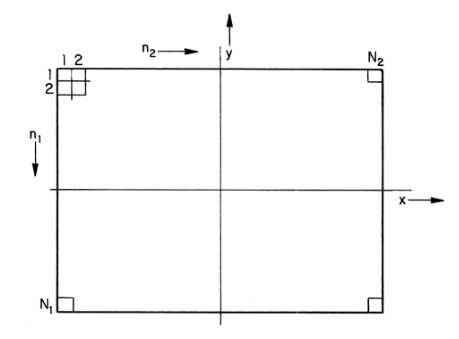
\includegraphics[width=0.6\textwidth]{figures/matrix} 
	\caption{Геометричний зв'язок між неперервним зображенням та його матрицею пікселів}
	\label{fig:matrix_geometry}
\end{figure}

Для зручності математичного аналізу матрицю зображення часто перетворюють у векторну форму. Це досягається шляхом послідовного сканування матриці $\mathbf{I}$ по стовпцях (або рядках) та об'єднання її елементів у один довгий вектор. Еквівалентну операцію сканування можна виразити у кількісній формі за допомогою операційного вектора $\mathbf{v}_j$ розмірністю $m \times 1$ та матриці $\mathbf{N}_j$ розмірністю $(n \cdot m) \times n$, що визначаються як:
\begin{equation}
	\mathbf{v}_j = 
	\begin{bmatrix}
		0 \\ \vdots \\ 0 \\ 1 \\ 0 \\ \vdots \\ 0
	\end{bmatrix}
	\begin{matrix}
		1 \\ \vdots \\ j-1 \\ j \\ j+1 \\ \vdots \\ m
	\end{matrix},
	\quad
	\mathbf{N}_j = 
	\begin{bmatrix}
		\mathbf{0} \\ \vdots \\ \mathbf{0} \\ \mathbf{E} \\ \mathbf{0} \\ \vdots \\ \mathbf{0}
	\end{bmatrix}
	\begin{matrix}
		1 \\ \vdots \\ j-1 \\ j \\ j+1 \\ \vdots \\ m
	\end{matrix}.
\end{equation}

Тоді векторне представлення $\mathbf{i}$ матриці зображення $\mathbf{I}$ отримується за допомогою операції зчеплення (stacking operation):
\begin{equation}
	\mathbf{i} = \sum_{j=1}^{m} \mathbf{N}_j \mathbf{I} \mathbf{v}_j.
\end{equation}

По суті, вектор $\mathbf{v}_j$ виділяє $j$-й стовпець із матриці $\mathbf{I}$, а матриця $\mathbf{N}_j$ розміщує цей стовпець у $j$-му сегменті довгого вектора $\mathbf{i}$. Таким чином, вектор $\mathbf{i}$ містить відскановані по стовпцях елементи матриці $\mathbf{I}$. Зворотне співвідношення для перетворення вектора $\mathbf{i}$ назад у матричну форму має вигляд:
\begin{equation}
	\mathbf{I} = \sum_{j=1}^{m} \mathbf{N}_j^T \mathbf{i} \mathbf{v}_j^T.
\end{equation}

Використовуючи ці оператори прямого та зворотного перетворення, можна легко переходити між векторним та матричним представленнями двовимірного масиву~\cite{pratt2014introduction}. Перехід до векторно-матричного представлення має принципове значення для алгоритмічної реалізації. Головна перевага такого підходу полягає у зведенні складних двовимірних просторових перетворень до стандартних операцій лінійної алгебри. Це не лише забезпечує компактну математичну нотацію, а й формує строгий аналітичний базис для подальшої математичної оптимізації алгоритму масштабування. Як буде показано далі, оперування зображенням у матричній формі дозволяє ефективно факторизувати інтерполяційні ядра, розпаралелювати обчислювальні процеси та застосовувати апаратно-прискорені інструкції на рівні програмного коду.